\documentclass[a4paper, 11px]{article}

\usepackage[french]{babel}
\usepackage[utf8]{inputenc}
\usepackage{fancyhdr}
\usepackage{lastpage}
\usepackage{graphicx}
\usepackage{rotating}
\usepackage{textcomp}
\usepackage{xspace}
\usepackage[toc,page]{appendix}
\usepackage{array}
\usepackage{amssymb}
\usepackage{enumerate}
\usepackage{enumitem}
\usepackage{eso-pic}

% \usepackage{needspace}


%%%%%%
 
\usepackage{listings}

\lstset{
  morekeywords={},
  sensitive=f,
  morecomment=[l]--,
  morestring=[d]",
  showstringspaces=false,
  basicstyle=\small\ttfamily,
  keywordstyle=\bf\small,
  commentstyle=\itshape,
  stringstyle=\sf,
  extendedchars=true,
  columns=[c]fixed
}

% CI-DESSOUS: conversion des caractères accentués UTF-8 
% en caractères TeX dans les listings...
\lstset{
  literate=%
  {À}{{\`A}}1 {Â}{{\^A}}1 {Ç}{{\c{C}}}1%
  {à}{{\`a}}1 {â}{{\^a}}1 {ç}{{\c{c}}}1%
  {É}{{\'E}}1 {È}{{\`E}}1 {Ê}{{\^E}}1 {Ë}{{\"E}}1% 
  {é}{{\'e}}1 {è}{{\`e}}1 {ê}{{\^e}}1 {ë}{{\"e}}1%
  {Ï}{{\"I}}1 {Î}{{\^I}}1 {Ô}{{\^O}}1%
  {ï}{{\"i}}1 {î}{{\^i}}1 {ô}{{\^o}}1%
  {Ù}{{\`U}}1 {Û}{{\^U}}1 {Ü}{{\"U}}1%
  {ù}{{\`u}}1 {û}{{\^u}}1 {ü}{{\"u}}1%
}

%%%%%%%%%%
% TAILLE DES PAGES (A4 serré)

\setlength{\parindent}{1cm}
\setlength{\parskip}{1ex}
\setlength{\textwidth}{17cm}
\setlength{\textheight}{22,7cm}
\setlength{\oddsidemargin}{-.7cm}
\setlength{\evensidemargin}{-.7cm}


\renewcommand{\labelenumi}{\arabic{enumi}.} 
\renewcommand{\labelenumii}{\arabic{enumi}.\arabic{enumii}}
\renewcommand{\labelenumiii}{\arabic{enumi}.\arabic{enumii}.\arabic{enumiii}}

%%%%%%%%%%

\newcommand\BackgroundPic{
\put(0,0){
\parbox[b][\paperheight]{\paperwidth}{%
\vfill

\includegraphics[width=\paperwidth,height=\paperheight,
keepaspectratio]{background.jpg}%
\vfill
}}}
%%%%%%%

\begin{document}

\AddToShipoutPicture{\BackgroundPic}


\renewcommand{\appendixtocname}{Annexes}
\DeclareGraphicsExtensions{.pdf,.png,.jpg}

\begin{titlepage}
\setlength{\parindent}{0cm}

\begin{center}

% Upper part of the page
\begin{figure}[!h]

\includegraphics[bb=-550 -10 -250 20, scale=0.7]{./logo.pdf}
\end{figure}
% logo.pdf: 612x792 pixel, 72dpi, 21.59x27.94 cm, bb=0 0 612 792


\vspace{4cm}
\rule{\linewidth}{.5pt}
\vspace{2mm}


\begin{center}
{\LARGE GRAND CERCLE MOBILE - GCM}

\vspace{1cm}


{\Huge \bf Spécifications Externes}


\end{center}


\vspace{1cm}

%===================================================================
\begin{center}
$ $\\
\large{ \textbf{Luiza CICONE - Jérémy KREIN - Jérémy LUQUET - Paul MAYER}}\\
\large{ \textbf{ISI - IF}}
$ $\\
\end{center}
\rule{\linewidth}{.5pt}


\vfill

% Bottom of the page

{\large Mai 2012}

\end{center}
\end{titlepage}

\tableofcontents

\newpage

\section{Cas d'utilisations}
\begin{figure}[h!]
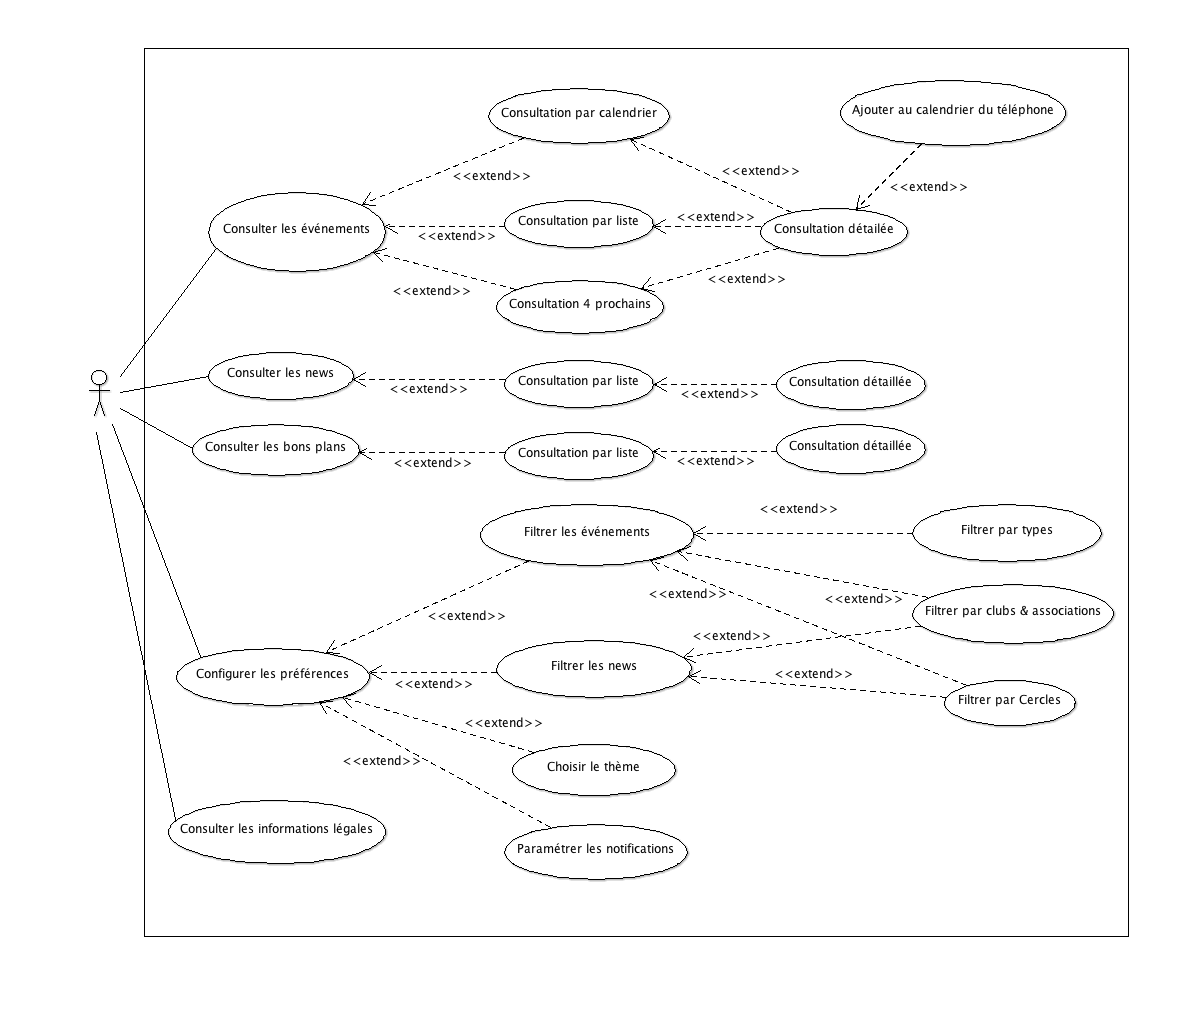
\includegraphics[width=20cm,height=15cm]{cas_utilisation.png}
\end{figure}

\newpage

\section{Modèle de tâches}
\vfill
\subsection{Fonctionnalités principales}
\begin{figure}[h!]
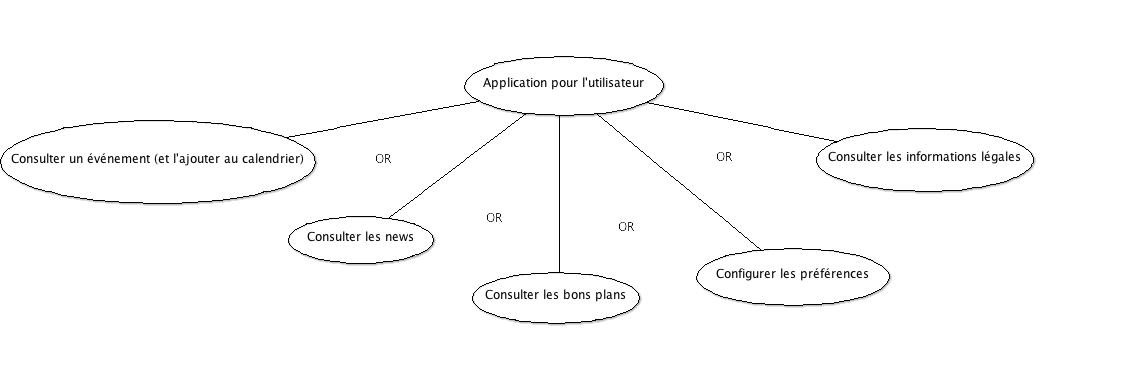
\includegraphics[width=18cm,height=8cm]{taches_generales.png}
\end{figure}

\subsection{Consulter les événements}
\begin{figure}[h!]
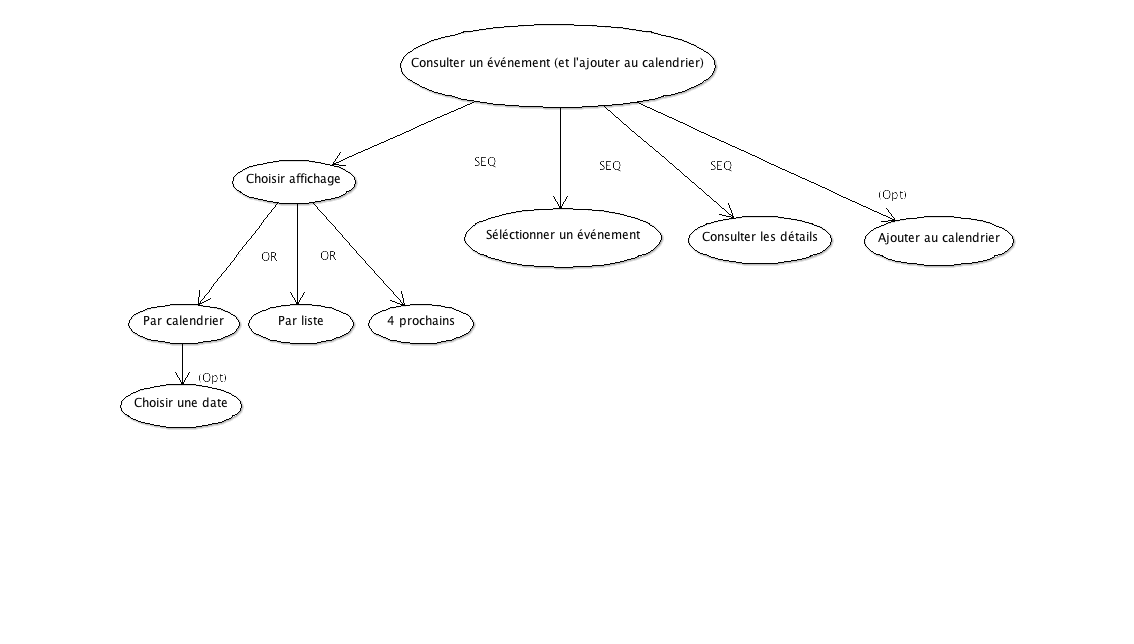
\includegraphics[width=20cm,height=15cm]{consulter_evenements.png}
\end{figure}
\vfill
\clearpage

\subsubsection{Ajouter au calendrier pour iOS}
\vfill
\begin{figure}[h!]
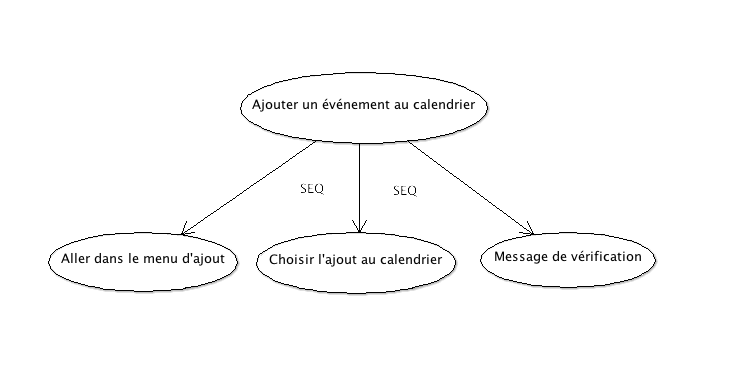
\includegraphics[width=18cm,height=8cm]{ajouter_evenement_calendrier_iOS.png}
\end{figure}

\subsubsection{Ajouter au calendrier pour Android}
\vfill
\begin{figure}[h!]
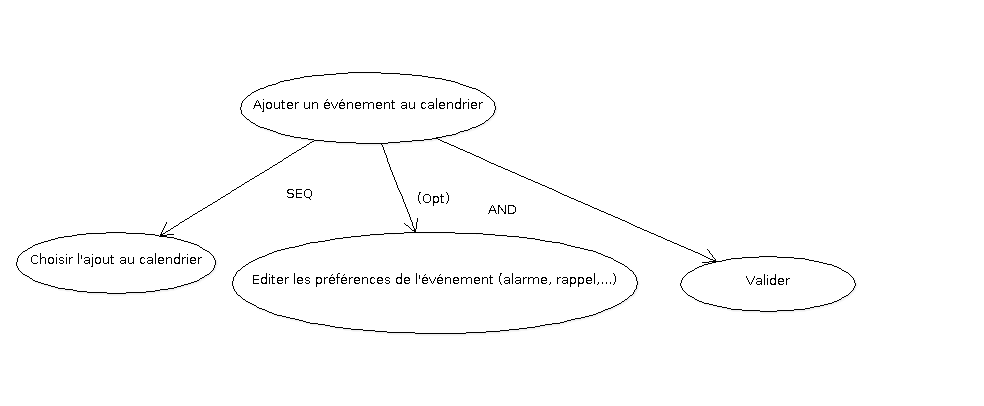
\includegraphics[width=18cm,height=8cm]{ajouter_evenement_calendrier_Android.png}
\end{figure}

\subsection{Consulter une news}
\vfill
\begin{figure}[h!]
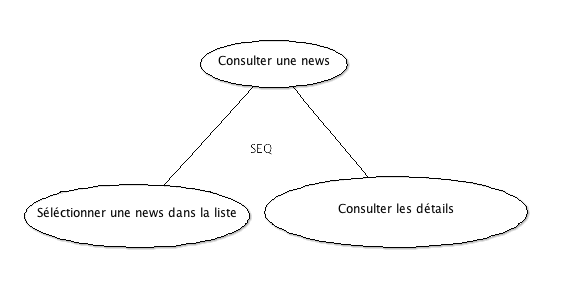
\includegraphics[width=18cm,height=8cm]{consulter_news.png}
\end{figure}

\subsection{Consulter un bon plan}
\vfill
\begin{figure}[h!]
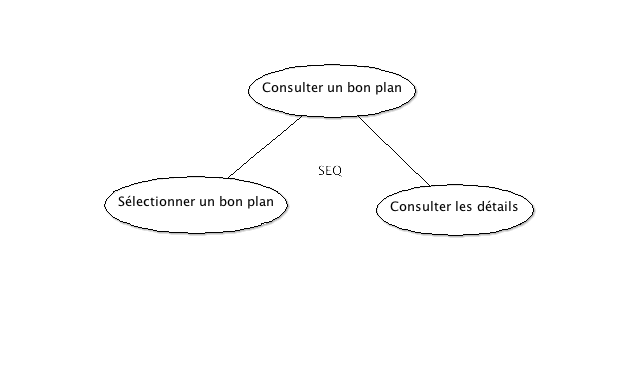
\includegraphics[width=18cm,height=8cm]{consulter_bonplans.png}
\end{figure}

\subsection{Configurer les préférences}
\begin{figure}[h!]
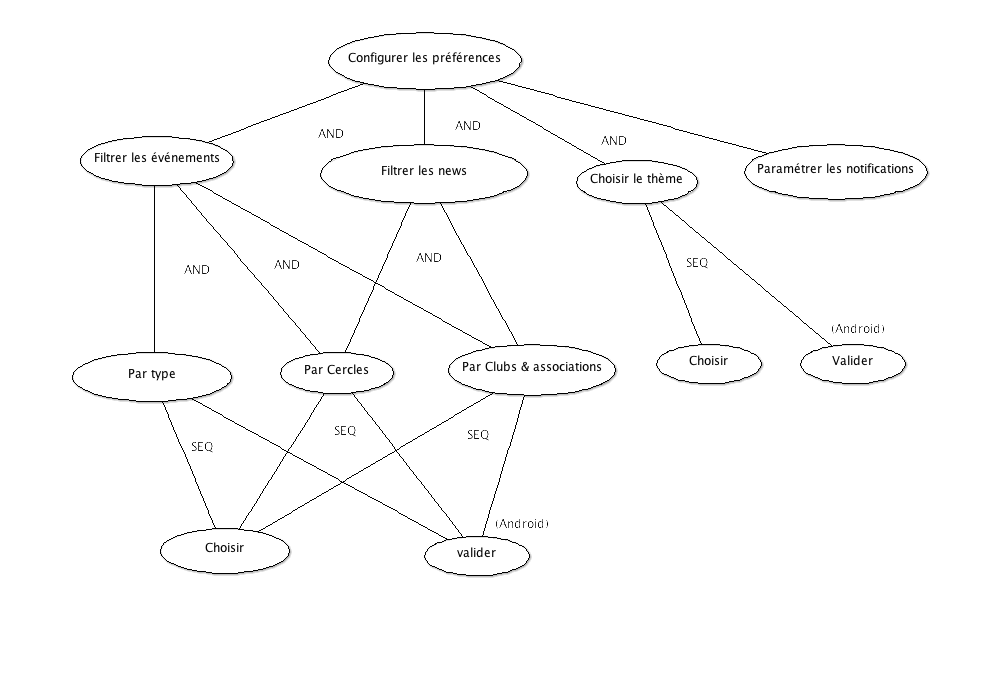
\includegraphics[width=20cm,height=15cm]{configurer_preferences.png}
\end{figure}
\vfill
\clearpage

\section{Diagrammes UML}

\newpage

\section{Interface utilisateur abstraite}

\newpage

\section{Sketching}

\subsection{Page 1}

\subsection{Page 2}

\subsection{Page 3}


\end{document}

